\scanpage{23}
$\mathcal G$ --- which therefore acts on $T$. This automatically gives rise \unsure{to|:}
\diagram{\begin{tikzcd}[ampersand replacement=\&,column sep=small]
\Phi:\unsure{\tau|\mathcal T}\&\unsure{\longrightarrow|\mathbin{-}}\&\operatorname{Hom}_{\mathrm{gr}}(T,\pi)\qquad\ldots
\end{tikzcd}}

That said, we have a homomorphism from the groupoid $\langle\unsure{\tau|\mathcal T},\pi\rangle$ into the groupoid of universal coverings of $\Pi$, constant on the objects and with value $\widetilde\Pi$ on these, which therefore sends the set of arrows into $\pi$ --- and which for $t,t'\in\unsure{\tau|\mathcal T}$, denoting by
\figure{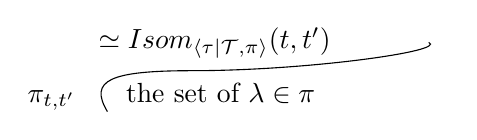
\begin{tikzpicture}[x=1cm,y=1cm]
\node[anchor=base west,inner sep=0pt] at (0,0) {$\pi_{t,t'}$};
\node[anchor=base west,inner sep=0pt] at (1.25,0) {the set of $\lambda\in\pi$};
\node[anchor=south west,inner sep=0pt] at (0.90,0.55) {\inserted{$\simeq\operatorname{Isom}_{\langle\unsure{\tau|\mathcal T},\pi\rangle}(t,t')$}};
\draw[thin] (1.02,-0.12) .. controls (0.78,0.28) and (1.05,0.40) .. (2.10,0.40) .. controls (3.55,0.40) and (5.35,0.65) .. (5.10,0.76);
\end{tikzpicture}}
such that $\lambda t=t'$, is the inclusion of $\pi_{t,t'}$ into $\pi$. This functor
\diagram{\begin{tikzcd}[ampersand replacement=\&]
\langle\unsure{\tau|\mathcal T},\pi\rangle\arrow[r]\&
\begin{gathered}
\text{Category of}\\
\text{universal coverings}\\
\text{of }\Pi\text{ equal}\\
\text{\unsure{to|:} }\widetilde\Pi\\
\simeq(\text{one object}\\
\text{and group of isomorphisms---}\\
\pi)
\end{gathered}
\end{tikzcd}}
is obviously compatible with action of $\unsure{\mathcal E|\Sigma}$ on $\unsure{\Pi|\widetilde\Pi}$ hence on $\pi\ldots.$
\mspage{22}
